% =====================================
% Dies ist eine LaTeX-Vorlage für Masterarbeiten und vergleichbare Abschlussarbeiten bei Professor Bialonski.
% Die Vorlage ist aus einer bei Professor Bialonski durchgeführten Masterarbeit hervorgegangen.
% 
% Die Vorlage enthält einige Beispielinhalte, -tabellen und -abbildungen, an denen die Nutzung der verschiedenen Pakete und allgemeine LaTeX-Kommandos zur Ausarbeitung einer Abschlussarbeit zu sehen sind.
% Diese erheben weder einen Anspruch auf Vollständigkeit noch darauf immer den aktuell als Best Practice angesehenen Standards zu folgen.
% 
% Stellen, an denen Entscheidungen über Konfigurationen, verwendete Pakete etc. getroffen werden müssen sind mit einem TODO gekennzeichnet.
% =====================================

% =====================================
% Tipps:
%   für die Nutzung mit einem Versionsverwaltungssystem sollte mindestens mit jedem neuen Satz eine neue Zeile angefangen werden
%   bei der Nutzung des Babel-Pakets mit ngerman kann mit "= ein Bindestrich eingefügt werden, der es LaTeX erlaubt auch an anderen Stellen als dem Bindestrich einen Zeilenumbruch einzufügen, und mit "~ ein geschützter Bindestrich eingefügt werden, d.h. dieser darf nicht als Zeilenumbruch verwendet werden
%   bei der Verwendung z.B. von TeXstudio kann das LanguageTool eingebunden werden, siehe dazu auch https://paulomarconi.github.io/blog/LanguageTool%2BTeXstudio%2BVSCode/ und https://dev.languagetool.org/http-server
%   viele hilfreiche Tipps findet man hier: https://www.semipol.de/posts/2018/06/latex-best-practices-lessons-learned-from-writing-a-phd-thesis/
% =====================================


% Dokumentklasse
% TODO: Dies sind die wichtigsten Einstellungen, die vor Beginn des Schreibprozesses auf jeden Fall festgelegt werden sollten!
%       ich habe die KOMA-Script Abwandlung der report Klasse genutzt und kann dies auch im Nachhinein empfehlen
%       für allgemeine Informationen und Best Practices bezüglich der Auswahl der Schriftgröße und darauf basierend der Seitenränder empfiehlt es sich das Kapitel 2 der KOMA-Script Dokumentation (https://www.ctan.org/pkg/koma-script) zumindest zum Teil durchzulesen
%       ich finde den zweiseitigen Modus angebracht, dies kann allerdings auch zu weiteren Fragen bezüglich der Seitenränder etc. führen; wird der einseitige Modus genutzt, können eventuell die diversen \cleardoubleoddpage Befehle entfernt werden
%       die Bindungskorrektur wird von KOMA-Script dazu genutzt, den Verlust von Papier bei der Bindung in die Wahl der Seitenränder einzubeziehen, 10-12mm sind hier angebracht; für die reine Betrachtung als PDF wäre eigentlich eine Bindungskorrektur von 0 korrekt, dies würde allerdings zwei unterschiedliche Versionen mit ganz anderen Seitenrändern erfordern, von einer solchen Unterscheidung würde ich also abraten
%       DIV ist der Mechanismus der KOMA-Script Klassen für die Bestimmung der Breite der Seitenränder; ein guter Wert kann über "DIV=calc" berechnet werden und aus der log-Datei ausgelesen werden, anschließend kann man davon ausgehend leichte Änderungen vornehmen; für eine Schriftgröße von 12pt und einer Bindungskorrektur von 12mm ist 10 ein guter Wert; alternativ kann das geometry Paket verwendet werden, siehe dazu auch diverse weitere TODOs
\documentclass[
	12pt, % Schriftgröße
	twoside, % zweiseitiger Modus
	ngerman, % deutsches Dokument
	BCOR=12mm, % Bindungskorrektur
	DIV=10, % Division (Anzahl Spalten/Zeilen pro Seite, bestimmt implizit Margins)
	bibliography=toc % Literatur zu Inhaltsverzeichnis hinzufügen
]{scrreprt}

% Variablen bezüglich des Titels, Autors und Subjects
\newcommand{\titleDocument}{Logging, Tracing {\fontfamily{bch}\selectfont \&} Monitoring - Verfahren zur Überwachung von Anwendungen}
\newcommand{\authorDocument}{Natalie Fritzen}
\newcommand{\subjectDocument}{Bachelorarbeit}
\newcommand{\locationDocument}{Niederkassel-Rheidt}
\newcommand{\dateDocument}{\today} % Alternativ z.B. 30.~September 2021

% grundsätzliche Informationen zum Dokument
\title{\titleDocument}
\author{\authorDocument}
\date{\dateDocument}

% Packete etc.
\usepackage{thesis}

\usepackage{lipsum} % TODO: nur für Beispieltext in summary.tex genutzt, wird nicht benötigt

% Besondere Trennungen (z.B. bei vereinzelter Nutzung englischer Begriffe ohne Nutzung des multilingualen Supports von babel)
\hyphenation{Kon-fi-denz Kon-fi-denz-wert Mus-kel-ak-ti-vi-tät}

\begin{document}
	% ============ Anfang =============
	% Titelseite
	\begin{titlepage}
	% TODO: wird das geometry Paket genutzt statt der Mechanismen aus KOMA-Skript, kann die folgende Zeile z.B. durch "\newgeometry{...}" ersetzt werden
	\typearea{100} % DVI auf 100 setzen für Titel (kleine Margins)
	\setlength{\parindent}{0pt} % keine Einrückung bei neuen Absätzen auf dieser Seite
	
	\begin{flushright}
		
\includegraphics[height=5cm]{images/FH-Aachen-r_svg-raw}
	\end{flushright}
	
	\vspace*{-2.5cm}

	\begin{center}
		\textbf{\Huge Fachhochschule~Aachen}

		\vspace*{0.5cm}
		
		\textbf{\Huge Campus~Köln}

		\vspace*{0.75cm}

		{\normalsize\doublespacing Fachbereich~9:~Medizintechnik~und~Technomathematik\\	Studiengang:~Angewandte~Mathematik~und~Informatik}

		\vspace*{2.5cm} % TODO: bei mehr verwendeten Zeilen für den Titel verringern
		
		\begin{minipage}[t]{17cm} % TODO: abhängig von dem konkreten Titel muss diese Breite eventuell angepasst werden für einen passenden Zeilenumbruch
			\begin{center}
				\textbf{\Huge \titleDocument}
			\end{center}
		\end{minipage}
	
		\vspace*{2.5cm} % TODO: bei mehr verwendeten Zeilen für den Titel verringern (symmetrisch zu oben)
		
		\textbf{\Large \subjectDocument}

		\vspace*{0.5cm}
		
		{\normalsize von}
		
		\vspace*{0.5cm}
		
		\textbf{\Large \authorDocument}
	
		\vspace*{3.5cm}
		
		\begin{minipage}[t]{13cm}
			\begin{center}
				\begin{tabular}{ll}
					Prüfer: & Prof. Dr. rer. nat. Karola Merkel \\
					Zweitprüfer: & B. Sc. Sebastian Otto \\
					Matrikelnummer: & 3240219 \\
				\end{tabular}
			\end{center}
		\end{minipage}
		
		\vspace*{2.5cm}
	
		{\large \locationDocument, den \dateDocument}
%		TODO: Datum der Abgabe
	\end{center}
\end{titlepage}

	
	% Eidesstattliche Erklärung und Abstrakt
	\begingroup
		% keine Seitenzahl und kein running header
		\thispagestyle{empty}
		\renewcommand*{\chapterpagestyle}{empty}
		
		\cleardoubleoddpage % Eidesstattliche Erklärung rechts, damit Unterschrift nicht durchdrückt
		\chapter*{Eidesstattliche Erklärung} % kein Eintrag im Inhaltsverzeichnis

Ich versichere hiermit, dass ich die vorliegende {\subjectDocument} mit dem Thema
\begin{quote}
	\textit{\titleDocument}
\end{quote}
selbstständig verfasst und keine anderen als die angegebenen Quellen und Hilfsmittel benutzt habe, wobei ich alle wörtlichen und sinngemäßen Zitate als solche gekennzeichnet habe.
Die Arbeit wurde bisher keiner anderen Prüfungsbehörde vorgelegt und auch nicht veröffentlicht.

\vspace*{2cm}

\begingroup
	\setlength{\parindent}{0pt} % keine Einrückung bei neuen Absätzen in diesem Bereich
	
	\locationDocument, den \dateDocument
	\bigskip
	\bigskip
	
	% gewünschte Breite der Unterschriftslinie
	\newlength{\widthbox}
	\settowidth{\widthbox}{\locationDocument, den \dateDocument}
	
	\makebox[\widthbox]{\hrulefill}\\
	\authorDocument
\endgroup

		
		\cleardoubleoddpage % Abstrakt rechts
		\chapter*{Abstract} % kein Eintrag im Inhaltsverzeichnis


		
		\glsresetall % alle bereits genutzten Akronyme wieder zurücksetzen
	\endgroup
	
	% Inhaltsverzeichnis
	\cleardoubleoddpage % Inhaltsverzeichnis rechts
	\thispagestyle{plain}
	\tableofcontents
	
	% =========== Hauptteil ===========
	\cleardoubleoddpage % Beginn Einleitung rechts
	\chapter{Einleitung} \label{ch:introduction}


	%\include{basics}
	%\include{data}
	%\include{methods}
	\chapter{Ergebnisse} \label{sec:results}

Nachfolgend ist eine Beispielabbildung und eine Beispieltabelle zu sehen.
Die Abbildung ist als \textit{svg}-Datei abgelegt und wird mit Inkscape automatisch in eine \textit{pdf}-Datei umgewandelt.

\begin{figure}
	\centering
	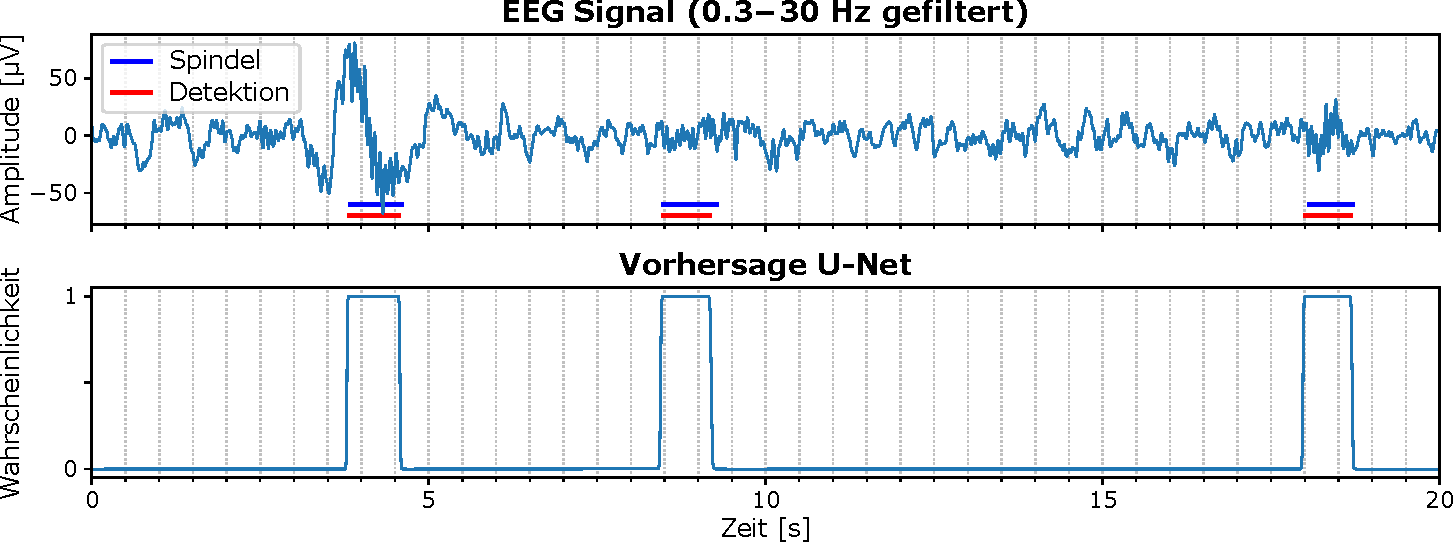
\includegraphics[width=\linewidth]{images/spindle-detection-u-net_svg-raw}
	\caption{
		Detektion des U"~Net Modells beispielhaft auf \SI{20}{\s} der Testdaten.
		In der ersten Zeile ist das Breitband"=Signal mit den annotierten und detektierten Spindeln und in der zweiten Zeile die vom Modell ausgegebene Wahrscheinlichkeit für eine Schlafspindel abgebildet.
	}
	\label{fig:results:spindle-detection-u-net}
\end{figure}

\begin{table}
	\centering
	\begin{threeparttable}
		% Tabellen ohne Nutzung von \rowstyle können ohne ^ und + angelegt werden
		\begin{tabular}{@{}^l+c+c+c+c+c+c+c+c+c@{}}
			\toprule
			& \multicolumn{3}{c}{beide Kohorten} & \multicolumn{3}{c}{jüngere Kohorte} & \multicolumn{3}{c}{ältere Kohorte} \\
			\cmidrule(l){2-4} \cmidrule(l){5-7} \cmidrule(l){8-10}
			Detektor & Recall & Prec & F1 & Recall & Prec & F1 & Recall & Prec & F1 \\
			\midrule
			Experte\tnote{1,2} & \num{0.72} & \num{0.78} & \num{0.72} & \num{0.76} & \num{0.81} & \num{0.76} & \num{0.66} & \num{0.74} & \num{0.65} \\
			A7 \autocite{Lacourse2019}\tnote{1} & \num{0.73} & \num{0.71} & \num{0.72} & \num{0.75} & \num{0.73} & \num{0.74} & \num{0.70} & \num{0.69} & \num{0.70} \\
			A7 \autocite{Lacourse2019}\tnote{3} & \num{0.76} & \num{0.70} & \num{0.73} & \num{0.78} & \num{0.70} & \num{0.74} & \num{0.73} & \num{0.69} & \num{0.71} \\
			\rowstyle{\color{red}}
			U-Net & \num{0.79} & \num{0.85} & \num{0.82} & \num{0.82} & \num{0.85} & \num{0.84} & \num{0.73} & \num{0.85} & \num{0.79} \\
			\bottomrule
		\end{tabular}
		\begin{tablenotes}
			\item[1]{Wie in \autocite{Lacourse2020} berichtet.}
			\item[2]{Durchschnittlicher Wert der Experten bezogen auf den Gruppenkonsens ohne den jeweiligen Experten.}
			\item[3]{Auf den hier genutzten Testdaten ausgewertet.}
		\end{tablenotes}
	\end{threeparttable}
	\caption{
		Ergebnisse auf den Testdaten bei der Evaluierung beider Kohorten und bei der Evaluierung jeweils einer Kohorte.
		Die Ergebnisse aus \autocite{Lacourse2020} sind auf allen $n=180$ Patienten berechnet worden, die hier verwendeten Testdaten umfassen $n=36$ Patienten.
		Angegeben sind jeweils Recall, Precision (\textit{Prec}) und F1 Score bei \SI{20}{\percent} Overlap Threshold.
	}
	\label{tab:results:f1-scores}
\end{table}


	\chapter{Zusammenfassung und Ausblick} \label{sec:summary}

Dies stellt das Ende dieses Templates dar \autocite{Surowiecki2005}.
Abschließend folgt Beispieltext für eine Visualisierung des Seitenlayouts etc.

\lipsum[1-18]{}

	
	% ============= Ende ==============
	\cleardoubleoddpage % Literaturverzeichnis rechts
	\printbibliography
\end{document}
